\section{Tomografiakuvan muodostus}
Kuvan rekonstruktiossa pyritään muodostamaan kuva radioaktiivisen merkkiaineen jakaumasta gammakameran havaitsemien fotonien perusteella\cite{cherry_single_2012, bruyant_analytic_2002, beister_iterative_2012, van_audenhaege_review_2015, bercovich_medical_2018}. Prosessissa voidaan kompensoida myös kuvaan vaikuttavia virhelähteitä, joista esimerkkeinä toimivat taustasäteily, laitteiston kalibrointivirheet, fotonien sironta ja potilaan liikkeet kuvantamisen aikana\cite{beister_iterative_2012, bruyant_analytic_2002}. Lopullisille tomografiakuville, joiden perusteella esimerkiksi diagnoosi tehdään, voidaan myös suorittaa jälkikäsittely suodattamalla tai muuttamalla kontrastia. Yleisesti jälkikäsittelyä ei kuitenkaan luokitella rekonstruktioksi, koska rekonstruktion keskiössä on kolmiulotteisen aktiivisuusjakauman määrittäminen.\cite{bruyant_analytic_2002}

Gammakameran perspektiivistä havaitaan ikään kuin kaksiulotteinen varjo radioaktiivisen merkkiaineen kolmiulotteisesta jakaumasta. Varjoista ei suoraan nähdä kuvattavan kohteen aktiivisuusjakaumaa, mutta keräämällä näitä projektioiksi kutsuttuja varjoja useasta suunnasta jakauma voidaan määrittää matemaattisin menetelmin.\cite{cherry_single_2012, bruyant_analytic_2002, beister_iterative_2012, van_audenhaege_review_2015, bercovich_medical_2018}. Samat matemaattiset menetelmät soveltuvat myös tietokonetomografiaan, jossa jokainen projektio vastaa tietystä suunnasta otettua tavallista röntgenkuvaa.

Projektioiden matematiikka esitetään kahdessa ulottuvuudessa (jolloin projektiot ovat yksiulotteisia) ymmärrettävyyden vuoksi. Yleistys kolmeen ulottuvuuteen ja kaksiulotteiseen projektioon on suhteellisen suoraviivainen.

Oletetaan toistaiseksi gammakameran kollimaattorin havaitsevan ainoastaan yhdestä suunnasta saapuvaa säteilyä ja tarkastellaan $xy$-tason jatkuvaa aktiivisuusjakaumaa $f\colon\RR^{2}\to\RR$. Olkoon $\theta$ gammakameran tangentin ja positiivisen $x$-akselin välinen kulma kuten \hyperref[fig:projektio]{kuvassa \ref*{fig:projektio}}. Merkitään projektiota $g(s, \theta)$, jossa $s$ on gammakameran tangentin suuntainen koordinaattiakseli.

\begin{figure}[H]
    \centering
    \captionsetup{width=.9\textwidth}
    \begin{tikzpicture}
    \draw[->, thick] (-3,0)--(3,0) node[right]{$x$};
    \draw[->, thick] (0,-3)--(0,3) node[above]{$y$};


    \begin{scope}[shift={(0, 0)}, rotate=30]
        \begin{scope}[shift={(0, 5)}, rotate=180] % Detektori
            \draw[->, thick] (3.5, -1.3) -- (-3.5, -1.3) node[right]{$s$}; % s-akseli
            \draw[domain=-1.5:1.5, smooth, variable=\s, red] plot ({\s}, {-2.3-cos(2 * pi / 3 * \s r)}) node[above left]{$g(s, \theta)$};

            % Kollimaattori
            \foreach \x in {-3.5, -3.2, ..., 3.5}
            \fill (\x,0) rectangle (\x + 0.1,1);
    
            % Tuikeaine
            \draw (-3.5, 0) rectangle (3.5, -1);
            \fill[pattern=north east lines] (-3.5, 0) rectangle (3.5, -1);
        \end{scope}
        % Aktiivisuusjakauma
        \fill[pattern=dots, pattern color=blue] (0,0) circle (1.5) node[below left]{$f(x, y)$};

        % Suora
        \draw[dashed, red] (0.9, -3) -- (0.9, 5);
    \end{scope}
\end{tikzpicture}
    \caption{Aktiivisuusjakauma $f$ $xy$-tasossa (siniset pisteet), gammakameran kollimaattori (mustat palkit), detektorin tuikeaine (väritetty alue) ja projektio $g(s, \theta)$, jossa $\theta$ on $s$- ja $x$-akseleiden välinen kulma. Yhteen projektion pisteeseen vaikuttava aktiivisuusjakauman osa on piirretty punaisella katkoviivalla. Kuva on muokattu lähteestä \cite{bruyant_analytic_2002}.}
    \label{fig:projektio}
\end{figure}

Kulmalla $\theta$ ja pisteessä $s$ gammakamera havaitsee säteilyä $xy$-tason suoralta $\Omega$, jonka määrittää
\begin{equation*}
    \Omega=\left\{ (x, y) \mid x\cos(\theta)+y\cos(\theta)=s \right\}.
\end{equation*}
Projektio, eli suoralta $\Omega$ havaittu säteily voidaan esittää siten Radon-muunnokseksi kutsuttuna polkuintegraalina\cite{radon_determination_1986, bruyant_analytic_2002}
\begin{equation}\label{eqn:radon-muunnos}
    g(s, \theta)=\int_{\Omega}f(x, y).
\end{equation}

Tietokoneella voidaan kuitenkin käsitellä ainoastaan äärellistä määrää mitattuja projektioita. Toisin sanoen muuttujat $s$ ja $\theta$ ovat diskreettejä, jonka vuoksi on luontevaa diskretoida muuttujat $x$ ja $y$ jakamalla kuva-alue pikseleihin (tai kolmiulotteisessa tapauksessa vokseleihin), joissa aktiivisuusjakaumat ovat vakioita.

\begin{figure}[H]
    \centering
    \captionsetup{width=.9\textwidth}
    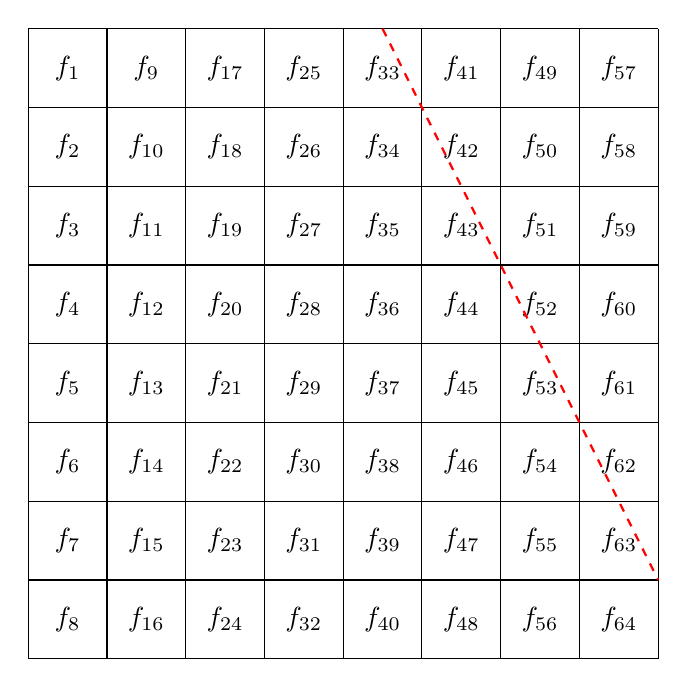
\begin{tikzpicture}
    % Vaakasuorat viivat
    \foreach \i in {0,1,...,8} {
        \draw (0, \i) -- (8, \i);
    }   

    % Pystysuorat viivat
    \foreach \j in {0,1,...,8} {
        \draw (\j, 0) -- (\j, 8);
    }

    % Pikselien indeksit
    \foreach \i in {0,1,...,7} {
        \foreach \j in {0,1,...,7} {
            \node at (\j+0.5, \i+0.5) {$f_{\the\numexpr \j*8 + (8 - \i) \relax}$};
        }
    }

    % Projektion suora
    \draw[thick, dashed, red] (4.5, 8) -- (8, 1);
\end{tikzpicture}
    \caption{Kuva-alue (ruudukko), kuva-alueen pikselit $f_i$, $i=1,\ldots,64$ ja projektion suora piirrettynä punaisella katkoviivalla.}
    \label{fig:diskreetti-projektio}
\end{figure}

%Kun kuva-alue jaetaan pikseleihin, joihin viitataan indekseillä $i=1,\ldots, n$, yhtälön (\ref{eqn:radon-muunnos}) integraali voidaan jakaa pikselikohtaisesti osiin
%\begin{alignat*}{2}
%    g(s, \theta)
%    &=\sum_{i=1}^{n}\int_{\Omega}f(x, y)\chi_{i}.
%\end{alignat*}
%

Oletetaan kuva-alueen aktiivisuusjakauma paloittain vakioksi pikselikohtaisesti. Tällöin voidaan merkitä
\begin{equation*}
    f(x, y)\chi_{i}=f_i.
\end{equation*}
Funktio $\chi_i$ on indikaattorifunktio, joka saa arvon 1 pikselin $i$ sisällä ja arvon 0 kaikkialla muualla. Yhtälön (\ref{eqn:radon-muunnos}) integraali palautuu summaksi
\begin{equation}\label{eqn:diskreetti-radon-muunnos}
    g(s, \theta)=\sum_{i=1}^{n}a_{i}f_{i},
\end{equation}
jossa $a_i$ on suoran $\Omega$ kulkema matka pikselissä $i$. 

\hyperref[fig:diskreetti-projektio]{Kuvassa \ref*{fig:diskreetti-projektio}} projektion suora kulkee kuva-alueen pikseleiden 33, 42, 43, 52, 53, 62 ja 63 lävitse. Suoran kulkema matka on jokaisessa edellä mainitusta pikselissä $\frac{\sqrt{5}}{2}$.

Koska kuva-alueen pikselien muodostama ruudukko on muodoltaan säännöllinen ja $\Omega$ on suora, niin kertoimet $a_i$ määräävät parametrit $s$ ja $\theta$ täysin. Merkitään tästä johtuen havaintojen lukumäärää vakiolla $m$, yhtä havaintoa vakiolla $g_i$, $0<i\leq m$ ja vastaavia kertoimia $a_{ij}$. Havainnot
\begin{equation*}
    \begin{cases}
        g_1&=\sum_{j=1}^{n}a_{1j}f_{j}\\
        &\vdots\\
        g_m&=\sum_{j=1}^{n}a_{mj}f_{j}
    \end{cases}
\end{equation*}
voidaan kerätä matriisiyhtälöön $g=Af$, jossa $g=\left( g_1, \ldots, g_m \right)^{T}$, $f=\left( f_1, \ldots, f_m \right)^{T}$ ja
\begin{equation*}
    A=
    \begin{pmatrix}
        a_{11} & a_{12} & \cdots & a_{1n} \\
        a_{21} & a_{22} & \cdots & a_{2n} \\
        \vdots & \vdots & \ddots & \vdots \\
        a_{m1} & a_{m2} & \cdots & a_{mn}
    \end{pmatrix}
\end{equation*}
on projektiomatriisi. Täsmällisempi nimitys matriisin $A$ operaatiolle on eteenpäinprojisointi, jonka lisäksi voidaan määritellä takaisinpäin projisointi. Tämä takaisinprojektio ikään kuin levittää projektiot $g$ takaisin kuva-alueelle. Aiemmin esitetyillä merkinnöillä ja oletuksilla takaisinprojektio on projektiomatriisin $A$ transpoosi.

Edellä kuvattu menetelmä on niin sanottu sädepohjainen projektio (\textit{ray-based projection}). OMEGAn toteutus sädepohjaisesta projektiosta perustuu Siddonin kehittämään algoritmiin\cite{wettenhovi_omegaopen-source_2021}. Algoritmissa määritetään aluksi säteen etenemissuunta ja leikkauspiste kuva-alueen reunan kanssa. Tästä eteenpäin hyödynnetään kuva-alueen säännöllisyyttä määrittämään yksi kerrallaan ne pikselit, joiden kautta säde kulkee. Samalla tallennetaan vastaavat säteen kuva-alueen pikseleissä kulkemat etäisyydet.\cite{siddon_fast_1985, sundermann_fast_1998}

Projektio voidaan laskea myös käyttämällä säteen sijasta sylinteriä ja laskemalla sylinterin ja vokseleiden leikkausten tilavuudet. Tässä tapauksessa vokselit oletetaan yleensä pallomaisiksi, jotta leikkauste tilavuudet olisivat nopeita laskea analyyttisesti.\cite{lougovski_volume_2014} Muissa projektion laskentaan käytetyissä menetelmissä hyödynnetään esimerkiksi kohtisuoraa etäisyyttä projektion säteen ja vokselin keskipisteen välillä\cite{aguiar_geometrical_2010} tai kuva-alueen taajuussisältöä\cite{zeng_frequency_1992, zeng_rotating_1994}. Taajuussisältöön perustuva menetelmä on laskennallisesti nopea ja eroaa muista myös siinä, että menetelmässä ajatellaan detektorin pysyvän paikoillaan kuva-alueen pyöriessä\cite{zeng_frequency_1992, zeng_rotating_1994}.

\subsection{Analyyttiset menetelmät}
Kuva-alueen aktiivisuusjakauma saadaan projektiosta yksinkertaisimmin takaisinprojektiolla, kuten \hyperref[fig:takaisinprojektio]{kuvassa \ref*{fig:takaisinprojektio}} on esitetty. Kuvassa projektioita on kerätty neljästä eri suunnasta ja projektiot ovat levitetty takaisin kuva-alueelle. Kuvan (a) aktiivisuusjakauman pisteet erottuvat kuvassa (b) selvästi tummempana.

\hyperref[fig:takaisinprojektio]{Kuvan \ref*{fig:takaisinprojektio}} alkuperäisen aktiivisuusjakauman ulkopuolella oleva punainen väritys havainnollistaa myös, kuinka takaisinprojektio ei kuitenkaan ole projektion käänteisoperaatio. Tästä syystä takaisinprojektiolla muodostettu kuva on sumea. Lisäksi jos projektioita on liian vähän, kuvaan voi esimerkiksi jäädä artefaktoina projektioiden suuntaisia viivoja.\cite{bruyant_analytic_2002, stiller_basics_2018}

\begin{figure}[H]
    \centering
    \captionsetup{width=.9\textwidth}
    \begin{subfigure}[t]{.4\textwidth}
        \resizebox{\linewidth}{!}{\begin{tikzpicture}
    \draw[black] (-6, -6) -- (-6, 6) -- (6, 6) -- (6, -6) -- cycle;
    \fill[pattern=dots, pattern color=blue] (1, 1) circle (0.5);
    \fill[pattern=dots, pattern color=blue] (-1, 1) circle (0.5);
    \fill[pattern=dots, pattern color=blue] (-1, -1) circle (0.5);
    \fill[pattern=dots, pattern color=blue] (1, -1) circle (0.5);
\end{tikzpicture}}
        \caption{Aktiivisuusjakauma}
    \end{subfigure}%
    \hspace*{.1\textwidth}
    \begin{subfigure}[t]{.4\textwidth}
        \resizebox{\linewidth}{!}{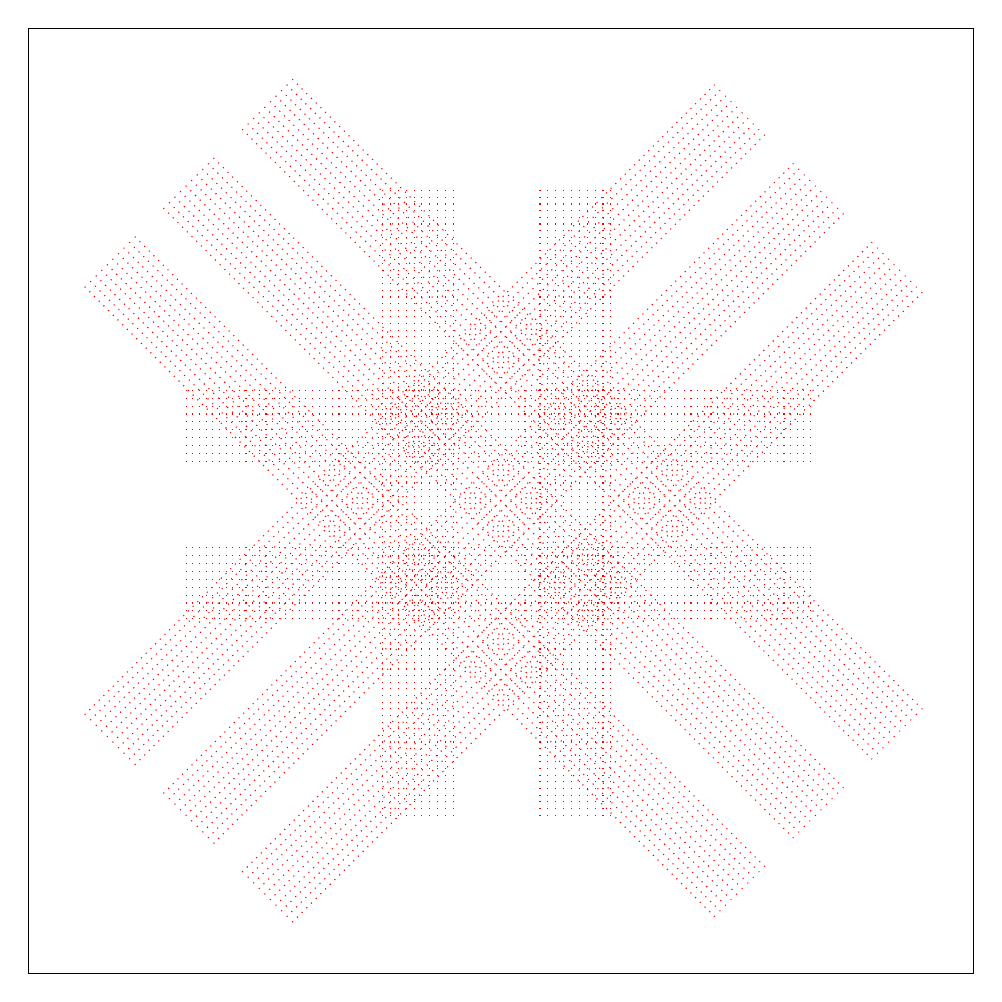
\begin{tikzpicture}
    \draw[black] (-6, -6) -- (-6, 6) -- (6, 6) -- (6, -6) -- cycle;
    \foreach \x in {-0.5, -0.4, ..., 0.5} {
        \draw[dotted, red] ({-1 + \x}, -4) -- ({-1 + \x}, 4);
        \draw[dotted, red] ({1 + \x}, -4) -- ({1 + \x}, 4);

        \draw[dotted, red] (-4, {-1 + \x}) -- (4, {-1 + \x});
        \draw[dotted, red] (-4, {1 + \x}) -- (4, {1 + \x});

        \draw[dotted, red] ({-4 - \x  / sqrt(2)}, {-4 + \x / sqrt(2)}) -- ({4 - \x / sqrt(2)}, {4 + \x / sqrt(2)});
        \draw[dotted, red] ({-4 - (\x+sqrt(2))  / sqrt(2)}, {-4 + (\x+sqrt(2)) / sqrt(2)}) -- ({4 - (\x+sqrt(2)) / sqrt(2)}, {4 + (\x+sqrt(2)) / sqrt(2)});
        \draw[dotted, red] ({-4 - (\x-sqrt(2))  / sqrt(2)}, {-4 + (\x-sqrt(2)) / sqrt(2)}) -- ({4 - (\x-sqrt(2)) / sqrt(2)}, {4 + (\x-sqrt(2)) / sqrt(2)});

        \draw[dotted, red] ({-4 - \x  / sqrt(2)}, {4 - \x / sqrt(2)}) -- ({4 - \x / sqrt(2)}, {-4 - \x / sqrt(2)});
        \draw[dotted, red] ({-4 - (\x+sqrt(2))  / sqrt(2)}, {4 - (\x+sqrt(2)) / sqrt(2)}) -- ({4 - (\x+sqrt(2)) / sqrt(2)}, {-4 - (\x+sqrt(2)) / sqrt(2)});
        \draw[dotted, red] ({-4 - (\x-sqrt(2))  / sqrt(2)}, {4 - (\x-sqrt(2)) / sqrt(2)}) -- ({4 - (\x-sqrt(2)) / sqrt(2)}, {-4 - (\x-sqrt(2)) / sqrt(2)});
    }
\end{tikzpicture}}
        \caption{Takaisinprojektio}
    \end{subfigure}%
    \caption{Takaisinprojektion idea. Vasemmalla puolella on sinisillä pisteillä piirretty aktiivisuusjakauma, josta on kerätty projektioita 4 eri suunnasta. Muodostaessa näistä takaisinprojektio, nähdään kuinka alkuperäisen aktiivisuusjakauman sijainti erottuu selvästi tummempana oikeanpuoleisessa kuvassa.}
    \label{fig:takaisinprojektio}
\end{figure}

Ratkaisuna tähän on kuvan taajuussisällön suodattaminen\cite{stiller_basics_2018, bruyant_analytic_2002}. Suodattaminen on mahdollista tehdä joko ennen (\textit{filtered backprojection, FBP}) tai jälkeen (\textit{backprojection filtering, BPF}) takaisinprojisoinnin, mutta yleensä suodatus tehdään ennen takaisinprojisointia.\cite{bruyant_analytic_2002}

Yleinen muoto projektioiden esittämiseen on sinogrammiksi kutsuttu matriisi. Sinogrammin sarakkeet vastaavat gammakameran detektorin pikseleitä ja rivit projektioita eri suunnista\cite{stiller_basics_2018}. Nimitys on peräisin siitä, kuinka yksittäinen pistemäinen säteilylähde näkyy sinogrammissa siniaaltona. FBP-algoritmissa sinogrammista suodatetaan pois matalat taajuudet, jolloin jäljelle jää korkeataajuuksiset yksityiskohdat. Tämä suodatettu sinogrammi takaisinprojisoidaan kuvaksi\cite{bruyant_analytic_2002}.

Analyyttisten menetelmien suurin etu on niiden nopeus, mutta niihin on kuitenkin hankalaa sisällyttää esitietoa kuvattavasta kohteesta, esimerkiksi säteilyn sironnasta. Menetelmä on myös altis kohinalle, koska kohina ilmenee pääosin jäljelle jäävissä korkeissa taajuuksissa.\cite{bruyant_analytic_2002, stiller_basics_2018}

\subsection{Iteratiiviset menetelmät}
Analyyttisissa menetelmissä kuva muodostetaan yleensä yhdellä takaisinprojisoinnilla, mutta iteratiiviisissa menetelmissä muodostettua kuvaa parannetaan toistuvasti vertaamalla mitattua projektiodataa jo muodostetun kuvan avulla simuloituihin eteenpäinprojektioihin. Jokainen iteratiivinen menetelmä lähtee liikkeelle arvauksesta, mitä aktiivisuusjakauma voisi olla. Arvaus on yleensä joko vakio tai esimerkiksi FBP:llä muodostettu kuva. Tämän jälkeen kaikissa iteratiivisissa menetelmissä on tietyt vaiheet, jotka ovat pääpiirteittäin\cite{bruyant_analytic_2002, beister_iterative_2012, stiller_basics_2018, ljungberg_spectct_2018}:
\begin{enumerate}[1.]
    \item Vaiheen 4 kuvasta (ensimmäisellä iteraatiolla alkuarvauksesta) lasketaan projektio. 
    \item Vaiheen 1 projektioita verrataan todellisiin, mitattuihin projektioihin. Näiden välisen eron, eli virheen, voidaan tulkita mittaavan kuinka paljon muodostettu kuva ja todellinen kuva eroavat toisistaan.
    \item Virhe takaisinprojisoidaan takaisin kuvaksi. 
    \item Arviota kuvasta päivitetään takaisinprojisoidun virheen perusteella.
    \item Tarkistetaan, kuinka paljon kuvan rekonstruktio on muuttunut edellisestä iteraatiosta. Jos ero ei ole riittävän pieni, siirrytään takaisin kohtaan 1. Vaihtoehtoisesti iteraatio voidaan pysäyttää tietyn enimmäismäärän jälkeen.
\end{enumerate}
Iteratiiviset algoritmit eroavat toisistaan lähinnä virheen muodostuksessa (vaihe 2) ja kuvan päivittämisessä (vaihe 4)\cite{bruyant_analytic_2002}.

Yleisimmin käytössä olevat iteratiiviset algoritmit ovat niin kutsuttuja tilastollisia algoritmeja, joissa havainnot $g_i$ tulkitaan satunnaismuuttujina $G_i\colon\mathbb{N}\to\mathbb{N}$\cite{wettenhovi_omegaopen-source_2021, kaipio_statistical_2005} ja projektiomatriisi tulkitaan projektiodatan todennäköisyysjakaumana\cite{boudjelal_novel_2021}. Edelleen, jokainen projektiomatriisin sarake vastaa yhtä kuva-alueen vokselia, mutta alkio $a_{ij}$ tulkitaan todennäköisyytenä, että hajoamistapahtuma vokselissa $i$ havaitaan indeksiä $j$ vastaavassa detektorissa\cite{boudjelal_novel_2021}.

Koska havaittujen hajoamistapahtumien määrä on pieni, positiivinen kokonaisluku, aktiivisuusjakaumaa voidaan mallintaa Poisson-jakaumalla\cite{kaipio_statistical_2005}. Projektiomatriisin avulla saadaan malli keskimääräiselle havainnolle $\overline{g}_i$, joka on muotoa\cite{boudjelal_novel_2021, shepp_maximum_1982}
\begin{equation*}
    \overline{g}_i=\sum_{j=1}^{n}a_{ij}f_j.
\end{equation*}
Siis
\begin{equation*}
    G_i\sim\text{Poisson}(\overline{g}_i),
\end{equation*}
eli havainnot ovat Poisson-jakautuneita keskiarvolla $\overline{g}_i$\cite{kaipio_statistical_2005, bruyant_analytic_2002, wettenhovi_transmission_2021}. Yleisesti Poisson-jakautuneen satunnaismuuttujan $X$ pistetodennäköisyysfunktio parametrilla $\lambda$ on
\begin{equation*}
    \pi(X=k)=e^{-\lambda}\frac{\lambda^{k}}{k!}.
\end{equation*}

Oletuksista seuraa, että todennäköisyys havaita $g_i$, kun tiedetään $f$, on
\begin{equation*}
    \pi(g_i \mid f)=e^{-\sum_{j=1}^{n}a_{ij}f_j}\frac{\left( \sum_{j=1}^{n}a_{ij}f_j \right)^{g_i}}{g_i!}.
\end{equation*}
Oletetaan satunnaismuuttujat $G_i$, $i=1,\ldots, m$, riippumattomiksi. Tällöin todennäköisyys sille, että havaitaan $g$ kun tiedetään $f$, on
\begin{equation*}
    \pi(g\mid f)=\prod_{i=1}^{m}e^{-\sum_{j=1}^{n}a_{ij}f_j}\frac{\left( \sum_{j=1}^{n}a_{ij}f_j \right)^{g_i}}{g_i!}.
\end{equation*}

Iteratiivisilla menetelmillä pyritään maksimoimaan todennäköisyys $\pi(g\mid f)$ kuvan $f$ suhteen. Yleensä kuitenkin etsitään maksimia funktiolle $\ln(\pi(g\mid f))$, koska maksimointimenetelmien johtaminen on tällöin helpompaa, eikä logaritmi vaikuta maksimikohdan sijaintiin. Shepp ja Vardi ovat artikkelissaan\cite{shepp_maximum_1982} osoittaneet maksimikohdan olemassaolon.

Emissiotomografiassa edellä mainitun kaltaisiin suurimman uskottavuuden (\textit{maximum likelihood}) estimaattoreihin pohjautuvista algoritmeista ensimmäinen on MLEM (\textit{maximum likelihood expectation maximization}), jossa arviota kuvasta päivitetään yhtälöllä\cite{boudjelal_novel_2021, shepp_maximum_1982, wettenhovi_omegaopen-source_2021, bruyant_analytic_2002, wettenhovi_transmission_2021}
\begin{equation*}
    f_j^{k+1}=\frac{f_j^{k}}{\sum_{i=1}^{m}a_{ij}}\sum_{i=1}^{m}\frac{a_{ij}g_i}{\sum_{j=1}^{n}a_{ij}f_j^{k}}.
\end{equation*}
MLEM-algoritmi kuitenkin suppenee verrattain hitaasti kohti maksimia ja on altis kohinalle\cite{wettenhovi_omegaopen-source_2021, bruyant_analytic_2002}. Jakamalla havainnot ja projektiomatriisi osajoukkoihin sekä käyttämällä MLEM-algoritmia jokaiseen osajoukkoon erikseen, saadaan algoritmi yleensä suppenemaan nopeammin. Eräs esimerkki tämän kaltaisesta menetelmästä on OSEM (\textit{ordered subsets expectation maximization}) ja sen muunnelmat.\cite{bruyant_analytic_2002, wettenhovi_omegaopen-source_2021, beister_iterative_2012}

\subsection{Virhelähteet kuvanmuodostuksessa}
Jokainen virhelähde voidaan mallintaa matriisimuodossa ja huomioida siten kuvan rekonstruktiossa. Käytännössä projektiomatriisia kerrotaan virhettä vastaavalla matriisilla. Puoli, jolta projektiomatriisia kerrotaan, riippuu siitä, kohdistuuko virheen korjaus projektiodataan vai kuvaan. Merkitään aiempien kappaleiden projektiomatriisia, jossa on huomioitu ainoastaan kuvantamisen geometria, matriisilla $G$. Merkitään esimerkiksi projektion mittaamisen epätarkkuutta matriisilla $H$ ja säteilyn vaimenemista matriisilla $B$. Nyt voidaan laskea projektiomatriisi
\begin{equation*}
    A=BGH,
\end{equation*}
jota käytettäessä kuvan rekonstruktiossa on huomioitu sekä epätarkkuus projektioiden havaitsemissa sekä säteilyn vaimeneminen\cite{wettenhovi_omegaopen-source_2021}.

Comptonin sironnasta ja valosähköisestä ilmiöstä johtuen gammasäteily vaimenee kulkiessaan aineen läpi. Vaimenemista kuvaa vaimenemiskerroin, joka riippuu gammafotonin energiasta ja aineen tiheydestä. Emissiotomografiassa fotonin energia on vakio, mutta aineen tiheys ja siten vaimenemiskerroin vaihtelee kudostyypin mukaan\cite{king_attenuation_2004, cherry_single_2012}. Tästä johtuen emissiotomografiaan yhdistetään yleensä transmissiotomografiakuvaus, jolla määritetään säteilyn vaimeneminen kuva-alueen vokseleissa\cite{king_attenuation_2004, cherry_single_2012, wettenhovi_omegaopen-source_2021}. Transmissiotomografiassa voidaan käyttää samaa detektoria kuin emissiotomografiassa. Tällöin transmissiotomografian gammafotonin energian täytyy kuitenkin poiketa emissiotomografiassa käytetyn fotonin energiasta, jotta havaittu fotoni voidaan tunnistaa transmissiotomografian fotoniksi. Transmissiotomografiakuvaa ei vaimenemiskertoimen energiariippuvuuden vuoksi voida käyttää vaimenemisen korjaukseen sellaisenaan, joten vaimenemiskertoimet skaalataan ennen vaimenemiskorjausta vastaamaan emissiotomografiassa käytetyn fotonin energiaa\cite{cherry_single_2012, king_attenuation_2004, wettenhovi_omegaopen-source_2021}.

Vaikka gammafotoni lähestyisi detektoria kollimaattorin reiän suuntaisesti, sen alkuperäisen etenemissuunnan on mahdollista olla jokin muu sironnan vuoksi. Tällä tavoin väärin havaittuja hajoamistapahtumia voi korjata useammalla tavalla. Yleisin tapa huomioida sironta on niin sanottujen energiaikkunoiden käyttäminen. Energiaikkunalla viitataan siihen energiaväliin, jolta detektorille saapuvat gammafotonit rekisteröidään. Sironneilla gammafotoneilla tämä energia on matalampi, joka tarkoittaa, että sironneista gammafotoneista voidaan mitata erilliset projektiot. Nämä projektiot skaalataan ja vähennetään kyseessä olevan isotoopin lähettämien gammafotonien energian ympärillä olevasta energiaikkunasta. Sironneille gammakvanteille voidaan käyttää myös useampia energiaikkunoita, mutta tällöin kussakin ikkunassa havaitaan vähemmän hajoamistapahtumia, lisäten kohinaa.\cite{cherry_single_2012, king_attenuation_2004} Kliinisiin sovelluksiin sopivaan tasapainoon laskenta-ajan ja kuvan laadun välillä riittää kaksi tai kolme energiaikkunaa\cite{king_attenuation_2004, cherry_single_2012}. 

Kohinalla viitataan siihen vaihteluun havainnoissa, joka ei anna hyödyllistä informaatiota kuvan rekonstruktiossa tai vaikeuttaa kuvan tulkintaa. Kohina voi olla joko satunnaista tai systemaattista, joista jälkimmäistä kutsutaan artifaktoiksi. Radioaktiivisen hajoamisen satunnaisuuden lisäksi satunnaista kohinaa syntyy ei-ideaalista laitteistosta, esimerkiksi detektorin havaitsemiskyvyn lämpötilariippuvuudesta ja gammafotonien sironnasta. Myös taustasäteily vaikuttaa kuvan kontrastiin etenkin ajallisesti lyhyissä mittauksissa.\cite{cherry_single_2012, king_attenuation_2004} Artifaktat voivat olla peräisin esimerkiksi kuvan rekonstruktioalgoritmista tai ylimääräisestä säteilylähteestä SPECT-laitteen läheisyydessä.

Muita erittelemisen arvoisia tekijöitä ovat säteilyn vaimeneminen ja sironta kollimaattorin reikien välisessä aineessa, ei-kohtisuorasti saapuvien gammakvanttien havaitsemisesta johtuva epätarkkuus aktiivisuusjakauman määrityksessä sekä epätarkkuudet tuikeaineessa syntyvän valon sijainnin paikantamisessa\cite{king_attenuation_2004, frey_collimator-detector_2006}. Edellä mainitut tekijät kootaan usein yhteen termin CDR (\textit{collimator-detector response}) alle. Kuvan rekonstruktiossa CDR:n voi huomioida joko mallintamalla sen analyyttisesti kollimaattorin ja detektorin geometrian avulla tai Monte Carlo -simulaatioilla, jotka ovat tarkempia mutta hitaampia.\cite{frey_collimator-detector_2006}

\subsection{OMEGA}
Tomografiakuvan rekonstruktioalgoritmien kehityksen ja kliinisen käyttöönoton hidasteeksi on tunnistettu helppokäyttöisten ja monipuolisten, mieluiten avoimen lähdekoodin, kehitysalustojen heikko saatavuus ja tehokkuus\cite{hutton_origins_2014}. Vaikka alustoja on kuitenkin olemassa useita, vuoteen 2021 asti ongelmana oli alustojen yhteentoimivuus eri laitteiston kanssa. Laitteistolla viitataan tässä yhteydessä tietokoneen keskusyksikköön (CPU) ja etenkin näytönohjaimeen (GPU), joilla kuvan rekonstruktio yleisimmin lasketaan. Ohjelmistot tukivat esimerkiksi näytönohjaimella laskettaessa ainoastaan CUDA-rajapintaa ja siten ainoastaan Nvidian näytönohjaimia.\cite{wettenhovi_omegaopen-source_2021}

OMEGA on avoimen lähdekoodin ohjelmisto tomografiakuvan rekonstruktioon, joka on kehitetty alkujaan PET-kuvan rekonstruktiota varten\cite{wettenhovi_omegaopen-source_2021, wettenhovi_transmission_2021}. Sittemmin ohjelmistoa on kehitetty tukemaan TT-kuvan rekonstruktiota\cite{wettenhovi_transmission_2021} ja tässä työssä toteuttava kollimaattorin mallinnus on tarkoitus sisällyttää tulevien versioiden SPECT-rekonstruktioon. OMEGA sisältää toteutukset yleisimmille estimaattoreille ja algoritmeille. Projektiot voidaan laskea joko sädepohjaisesti\cite{siddon_fast_1985, sundermann_fast_1998}, vokselin ja säteen kohtisuoralla etäisyydellä\cite{aguiar_geometrical_2010} tai kuva-alueen rotaatioon ja taajuussisältöön perustuvalla menetelmällä\cite{zeng_frequency_1992, zeng_rotating_1994}.\cite{wettenhovi_omegaopen-source_2021}

Ohjelmiston voidaan ajatella koostuvan kolmesta päällekkäisestä abstraktiokerroksesta, joissa ylhäältä alaspäin laskentateho kasvaa koodin luettavuuden kustannuksella. Kerroksia ja niiden toiminnallisuuksia on visualisoitu \hyperref[fig:omega-kerrokset]{kuvassa \ref*{fig:omega-kerrokset}}.

Ensimmäinen, ylin kerros koostuu MATLAB-koodista, joka on ajettavissa ilman kääntämistä sekä MATLAB-ohjelmistolla että avoimen lähdekoodin Octave-ohjelmistolla. Tällä kerroksella voidaan esimerkiksi suorittaa joitakin rekonstruktioalgoritmeista keskusyksiköllä ja käsitellä projektiodataa. Kerros on ainut käyttäjän eksplisiittisesti tarvitseva ja kerroksen toiminnallisuutta on myös verrattain helppo muokata sovelluskohteen mukaan.\cite{wettenhovi_transmission_2021, wettenhovi_omegaopen-source_2021}

\begin{figure}[H]
    \centering
    \captionsetup{width=.9\textwidth}
    \resizebox{.9\linewidth}{!}{
        \tikzstyle{kerros} = [rectangle, draw=black, rounded corners, minimum width=12cm, minimum height=1cm, text centered, font=\normalsize, line width=1]
\tikzstyle{palikka} = [rectangle, draw=black, minimum width=2.5cm, minimum height=1cm, text centered, font=\normalsize, line width=1, align=center]
\tikzstyle{nuoli} = [thick, draw=black, line width=1, ->, >=stealth]
\begin{tikzpicture}[node distance=2cm]
    \node (kerros1) [kerros, minimum width=14cm] {MATLAB / Octave};
    \node (data1) [below of=kerros1, xshift=1cm, palikka] {Datan käsittely};
    \node (rekonstruktio1) [left of=data1, xshift=-2cm, palikka] {Kuvan rekonstruktio};
    
    \node (kerros2) [below of=data1, kerros] {C++};
    \node (data2) [below of=kerros2, palikka] {Datan käsittely};
    \node (projektiomatriisi) [right of=data2, xshift=2cm, palikka] {Projektiomatriisin\\muodostus};
    \node (rekonstruktio2) [left of=data2, xshift=-2cm, palikka] {Kuvan rekonstruktio};
    
    \node (kerros3) [below of=data2, kerros] {OpenCL / CUDA};
    \node (rekonstruktio3) [below of=kerros3, palikka] {Kuvan rekonstruktio};
    
    \draw [nuoli] ([xshift=1cm]kerros1.south) -- (data1);
    \draw [nuoli] (data1) -- (kerros2);
    \draw [nuoli] (data1) -- (rekonstruktio1);
    \draw [nuoli] (rekonstruktio1) -- ([xshift=-3cm]kerros1.south);

    \draw [nuoli] ([xshift=3.5cm]kerros2.south) -- ([xshift=-.5cm]projektiomatriisi.north);    
    \draw [nuoli] ([xshift=.5cm]projektiomatriisi.north) -- ([xshift=4.5cm]kerros2.south);
    \draw [nuoli] ([xshift=-4cm]kerros2.south) -- (rekonstruktio2);
    \draw [nuoli] (kerros2.south) -- (data2);
    \draw [nuoli] ([xshift=.5cm]data2.south) -- ([xshift=.5cm]kerros3.north);
    \draw [nuoli] (rekonstruktio2.west) -| ([xshift=-5.5cm]kerros1.south);
    \draw [nuoli] ([xshift=-.5cm]data2.south) |- ([yshift=-.5cm]rekonstruktio2.south) -| ([xshift=-6cm]kerros1.south);

    \draw [nuoli] (kerros3) -- (rekonstruktio3);
    \draw [nuoli] (rekonstruktio3.west) -| ([xshift=-6.5cm]kerros1.south);
\end{tikzpicture}
    }
    \caption{OMEGA-ohjelmiston kerrokset (pyöreäkulmaiset laatikot) ja niiden tärkeimmät toiminnallisuudet (teräväkulmaiset laatikot). Kuva on muokattu lähteestä \cite{wettenhovi_omegaopen-source_2021}.}
    \label{fig:omega-kerrokset}
\end{figure}

OMEGAn toinen kerros sisältää C++-koodia, joka on käännetty MEX-tiedostoksi. Kerros sisältää esimerkiksi menetelmiä kuvan rekonstruktioon, datan käsittelyyn sekä projektiomatriisin laskemiseen.\cite{wettenhovi_transmission_2021, wettenhovi_omegaopen-source_2021} MATLAB-ohjelmiston MEX (MATLAB Executable) -tiedostot koostuvat käännetystä C-, C++- tai Fortran-koodista, joka on suoritettavissa MATLAB-ympäristössä. MEX-tiedostojen etuja ovat muun muassa parempi suorituskyky verrattuna perinteisiin MATLAB-tiedostoihin ja olemassa olevan C-, C++ tai Fortran-koodin hyödyntäminen. Kuvan rekonstruktion vaatiessa runsaasti laskentatehoa on luontevaa käyttää toiminnallisuutta hyödyksi.

Alin ja kaikista tehokkain kerros keskittyy kuvan rekonstruktioon OpenCL- ja CUDA-rajapinnoilla\cite{wettenhovi_transmission_2021, wettenhovi_omegaopen-source_2021}. Kuten aiemmin esitettiin, CUDA tukee ainoastaan Nvidian näytönohjaimia, mutta OpenCL:n etuna on tuki käytännössä kaikille moderneille moniydinsuorittimille ja näytönohjaimille valmistajasta riippumatta\cite{stone_opencl_2010}.